\documentclass[11pt,a4paper]{article}
\usepackage{fontspec}
\setmainfont{TeX Gyre Pagella}
\newfontfamily\headfont{Inter}[UprightFont=*-ExtraBold,BoldFont=*-ExtraBold,Extension=.otf,Path=/usr/share/fonts/opentype/inter/]
\usepackage[a4paper,margin=2.3cm]{geometry}
\usepackage{graphicx,booktabs,float,caption,array,xcolor,longtable}
\usepackage{xurl}
\usepackage[hidelinks]{hyperref}
\usepackage{titlesec}
\usepackage[round]{natbib}
\usepackage{setspace}
\setstretch{1.05}
\renewcommand{\topfraction}{0.9}
\renewcommand{\bottomfraction}{0.8}
\renewcommand{\textfraction}{0.1}
\renewcommand{\floatpagefraction}{0.75}
\setlength{\parindent}{0pt}
\setlength{\parskip}{0.55em}
\titleformat{\section}{\headfont\Large}{\thesection}{0.8em}{}
\titleformat{\subsection}{\headfont\large}{\thesubsection}{0.8em}{}
\captionsetup{font=small,labelfont=bf}
\urlstyle{same}
\hypersetup{pdftitle={How Fast Did News Travel?},pdfauthor={Tristan Hotham}}

\begin{document}
\begin{center}
{\Large\bfseries How Fast Did News Travel?\par}
\vspace{0.4em}
{\large Four American stories in 936 digitised newspapers, 1865 to 1941\par}
\vspace{1.2em}
{\large Tristan Hotham\par}
\vspace{0.3em}
{\small Independent researcher\\
ORCID: 0000-0003-4931-9349\\
DOI: https://doi.org/10.5281/zenodo.24052721\par}
\vspace{0.8em}
2026
\end{center}

\begin{quote}
\small
\begin{center}\textbf{Abstract}\end{center}
How long did it take for news to reach the American press, and what slowed it down? I measure, for every newspaper in a large digitised sample, the first issue that reported four national stories: the shooting of Abraham Lincoln (1865), the defeat of Custer's command at the Little Bighorn (1876), the sinking of the Titanic (1912) and the attack on Pearl Harbor (1941). The pages come from the American Stories dataset, structured OCR text of the Library of Congress's Chronicling America scans (13,233 issues of 936 papers in the event windows). A page counts as a report when it names the event after the earliest possible date and its text round the name contains a word about the event; 290 first reports were read by hand. Daily papers printed Lincoln's death, the Titanic and Pearl Harbor with the same median delay of one day: the telegraph had already removed distance as a cause of delay among connected cities by 1865, and later technologies did not shorten it further for the daily press. Weekly papers, the majority of the sample, waited for their press day (median 7, 4 and 5 days). Distance from the source explains almost nothing among dailies. The exceptions are informative: papers in the states of the former Confederacy took a median of 11 days to print Lincoln's death against 6 elsewhere, and no paper in the sample printed Custer's defeat until 11 days after the battle, after which it appeared in 12 papers in 9 states and territories on a single day. The slow step was the first mile to the wire, and the last step to the weekly press, not the distance between.

\textbf{Keywords:} history of news; telegraph; newspapers; Chronicling America; American Stories; diffusion of information; digital history
\end{quote}

\section{Introduction}
The speed of news is one of the classic measures of how connected a society is. Historians of communication have used the arrival dates of news in different towns to map the reach of the post, the railway and the telegraph \citep{pred1973}, and the telegraph in particular has been described as the moment when news first moved faster than people \citep{standage1998,blondheim1994}. Most such studies follow a handful of papers by hand. Large digitised newspaper archives now allow the same question to be asked of hundreds of papers at once.

This study takes four stories that every American newspaper would have printed and asks, for each paper in a large digitised sample, how many days passed between the event and its first report. The events span the telegraph age to the radio age: Lincoln's assassination in 1865, at the end of the Civil War; Custer's defeat at the Little Bighorn in 1876, on the northern plains far from any telegraph office; the Titanic disaster in 1912, the first great news story carried ashore by wireless; and the attack on Pearl Harbor in 1941, announced by radio within hours. It accompanies an interactive map that plays each story day by day (\url{https://maps.tristanhotham.com/news-speed/}).

\section{Data}
\textbf{American Stories.} The American Stories dataset \citep{dell2023} is structured text extracted from the page scans of Chronicling America, the Library of Congress's archive of digitised historic newspapers \citep{chronam}. A layout model finds the articles, headlines and captions on each page and OCR turns them into text; the dataset is released under CC BY 4.0. For each event I used every page in a window starting on the day of the event and running for six to ten weeks. Pages whose text matched the event's name (Lincoln, Custer, Titanic or Pearl Harbor) were kept with a snippet of about 180 characters round the first match; pages without a match were kept as one row per paper and date, which is enough to know which issues exist. In all the windows hold 13,233 issues of 936 newspapers and 14,941 pages that name an event.

\textbf{Places.} Each paper's Library of Congress title ends with its place of publication, for example ``(Columbus, Ohio) 1855-1870''. I matched the city and state to Wikidata's list of US cities, towns and villages \citep{wikidata}, preferring the most populous place of that name in the state, with GeoNames' list of places of 500 or more people \citep{geonames} as a fallback for large cities the Wikidata extract lacked and a short list of documented renamings (Yorkville, South Carolina is now York; Mechanicstown, Maryland is now Thurmont). Where the title gave no place, a town name inside the paper's own name was used if it matched a place of 200 or more people in the paper's state (The Waterbury Democrat, the Omaha Daily Bee). 772 papers were placed from their title, 78 from their name (two of them, where the name pointed to the wrong town, from the Library of Congress catalogue record instead) and 86 could not be placed; these are kept in every count that does not need a location.

\section{Methods}
\subsection{What counts as a report}
A name is not a story. Lincoln County, Custer City in the Black Hills and the ``titanic struggle'' of the war were all in print before each event. A page counts as reporting the event only if (1) it is dated on or after the first day the news could have been printed (15 April 1865; 3 July 1876, three days before the first report found anywhere in the sample; 15 April 1912; 7 December 1941) and (2) its snippet contains a word about the event itself from a list for each event (for Lincoln: assassination, shot, murder, death, funeral, mourning, Booth and so on; for Custer: massacre, killed, Sitting Bull, Little Horn, Reno, Sioux, troops; for the Titanic: iceberg, sank, disaster, Carpathia, survivors, in English, German, Spanish and other languages of the immigrant press; for Pearl Harbor: attack, bomb, Japanese, war, navy). The lists are matched on the raw text because the OCR glues line breaks to the following word.

\subsection{Hand review}
For each paper the earliest qualifying page decides its report date, so errors there matter most. I read the snippet of every first report that fell on the earliest possible day or the day after, that lacked a strong word, or that contained a phrase marking another use of the name (290 snippets) and rejected 9, for example an Artemus Ward sketch about a ``threatened assassination'' of Lincoln printed on 15 April and a letter from Custer City on 4 July. Rejections and acceptances are kept in a file in the code. In a random sample of 60 first reports that the review did not cover, 59 were plainly about the event and 1 was unclear.

\subsection{Delay, issues missed and publication rhythm}
For each paper and event I take the first issue dated on or after the floor date and the first issue that reports the event. The delay is the number of calendar days from the event to that report (so a morning paper of 15 April 1865 has a delay of one day, and an evening paper of 15 April 1912 a delay of none). The issues missed are the paper's digitised issues between the two. A paper is counted for an event if it has a digitised issue within 14 days of the floor date (145, 216, 566 and 69 papers). A paper is called daily if the median gap between its issues in the window is at most two days, weekly if it is five days or more, and otherwise ``several a week''. Distances are great-circle distances from where the news entered the national wires: Washington for 1865 and 1941, the battlefield for 1876 and New York for 1912. Relations between delay and distance are summarised with Spearman's rank correlation.

\section{Results}
\subsection{The four stories}
Table~\ref{tab:events} summarises the four events and Figure~\ref{fig:maps} maps every placed paper. Of the papers with an issue in the first fortnight, 93\% printed Lincoln's death within the window, 86\% Custer's defeat, 88\% the Titanic and 62\% Pearl Harbor (the last is low because many papers wrote of ``Hawaii'' or ``the war'' without naming the harbour, which the name match cannot see). The median delay was 7 days for Lincoln, 18 for Custer, 4 for the Titanic and 4 for Pearl Harbor.

\begin{table}[tbp]\centering\footnotesize\caption{The four events. Papers: with any digitised issue in the window; counted: with an issue within 14 days of the floor date. Reported: share of counted papers with a report in the window. Medians in days from the event, among reporting papers (in brackets, the number of counted daily or weekly papers). First issue: share of reporting papers that reported in their first issue after the floor date. By day 7: share of counted papers that had reported by day 7.}\label{tab:events}\begin{tabular}{lrrrrrrrr}\toprule Event & Papers & Counted & Reported \% & Median & Daily & Weekly & First issue \% & By day 7 \%\\\midrule
Lincoln shot, 1865 & 159 & 145 & 93 & 7 & 1 (24) & 7 (115) & 62 & 59\\
Little Bighorn, 1876 & 231 & 216 & 86 & 18 & 12 (35) & 18 (173) & 22 & 0\\
Titanic, 1912 & 589 & 566 & 88 & 4 & 1 (94) & 4 (450) & 65 & 64\\
Pearl Harbor, 1941 & 71 & 69 & 62 & 4 & 1 (12) & 5 (52) & 65 & 46\\
\bottomrule\end{tabular}\end{table}

\begin{figure}[tbp]\centering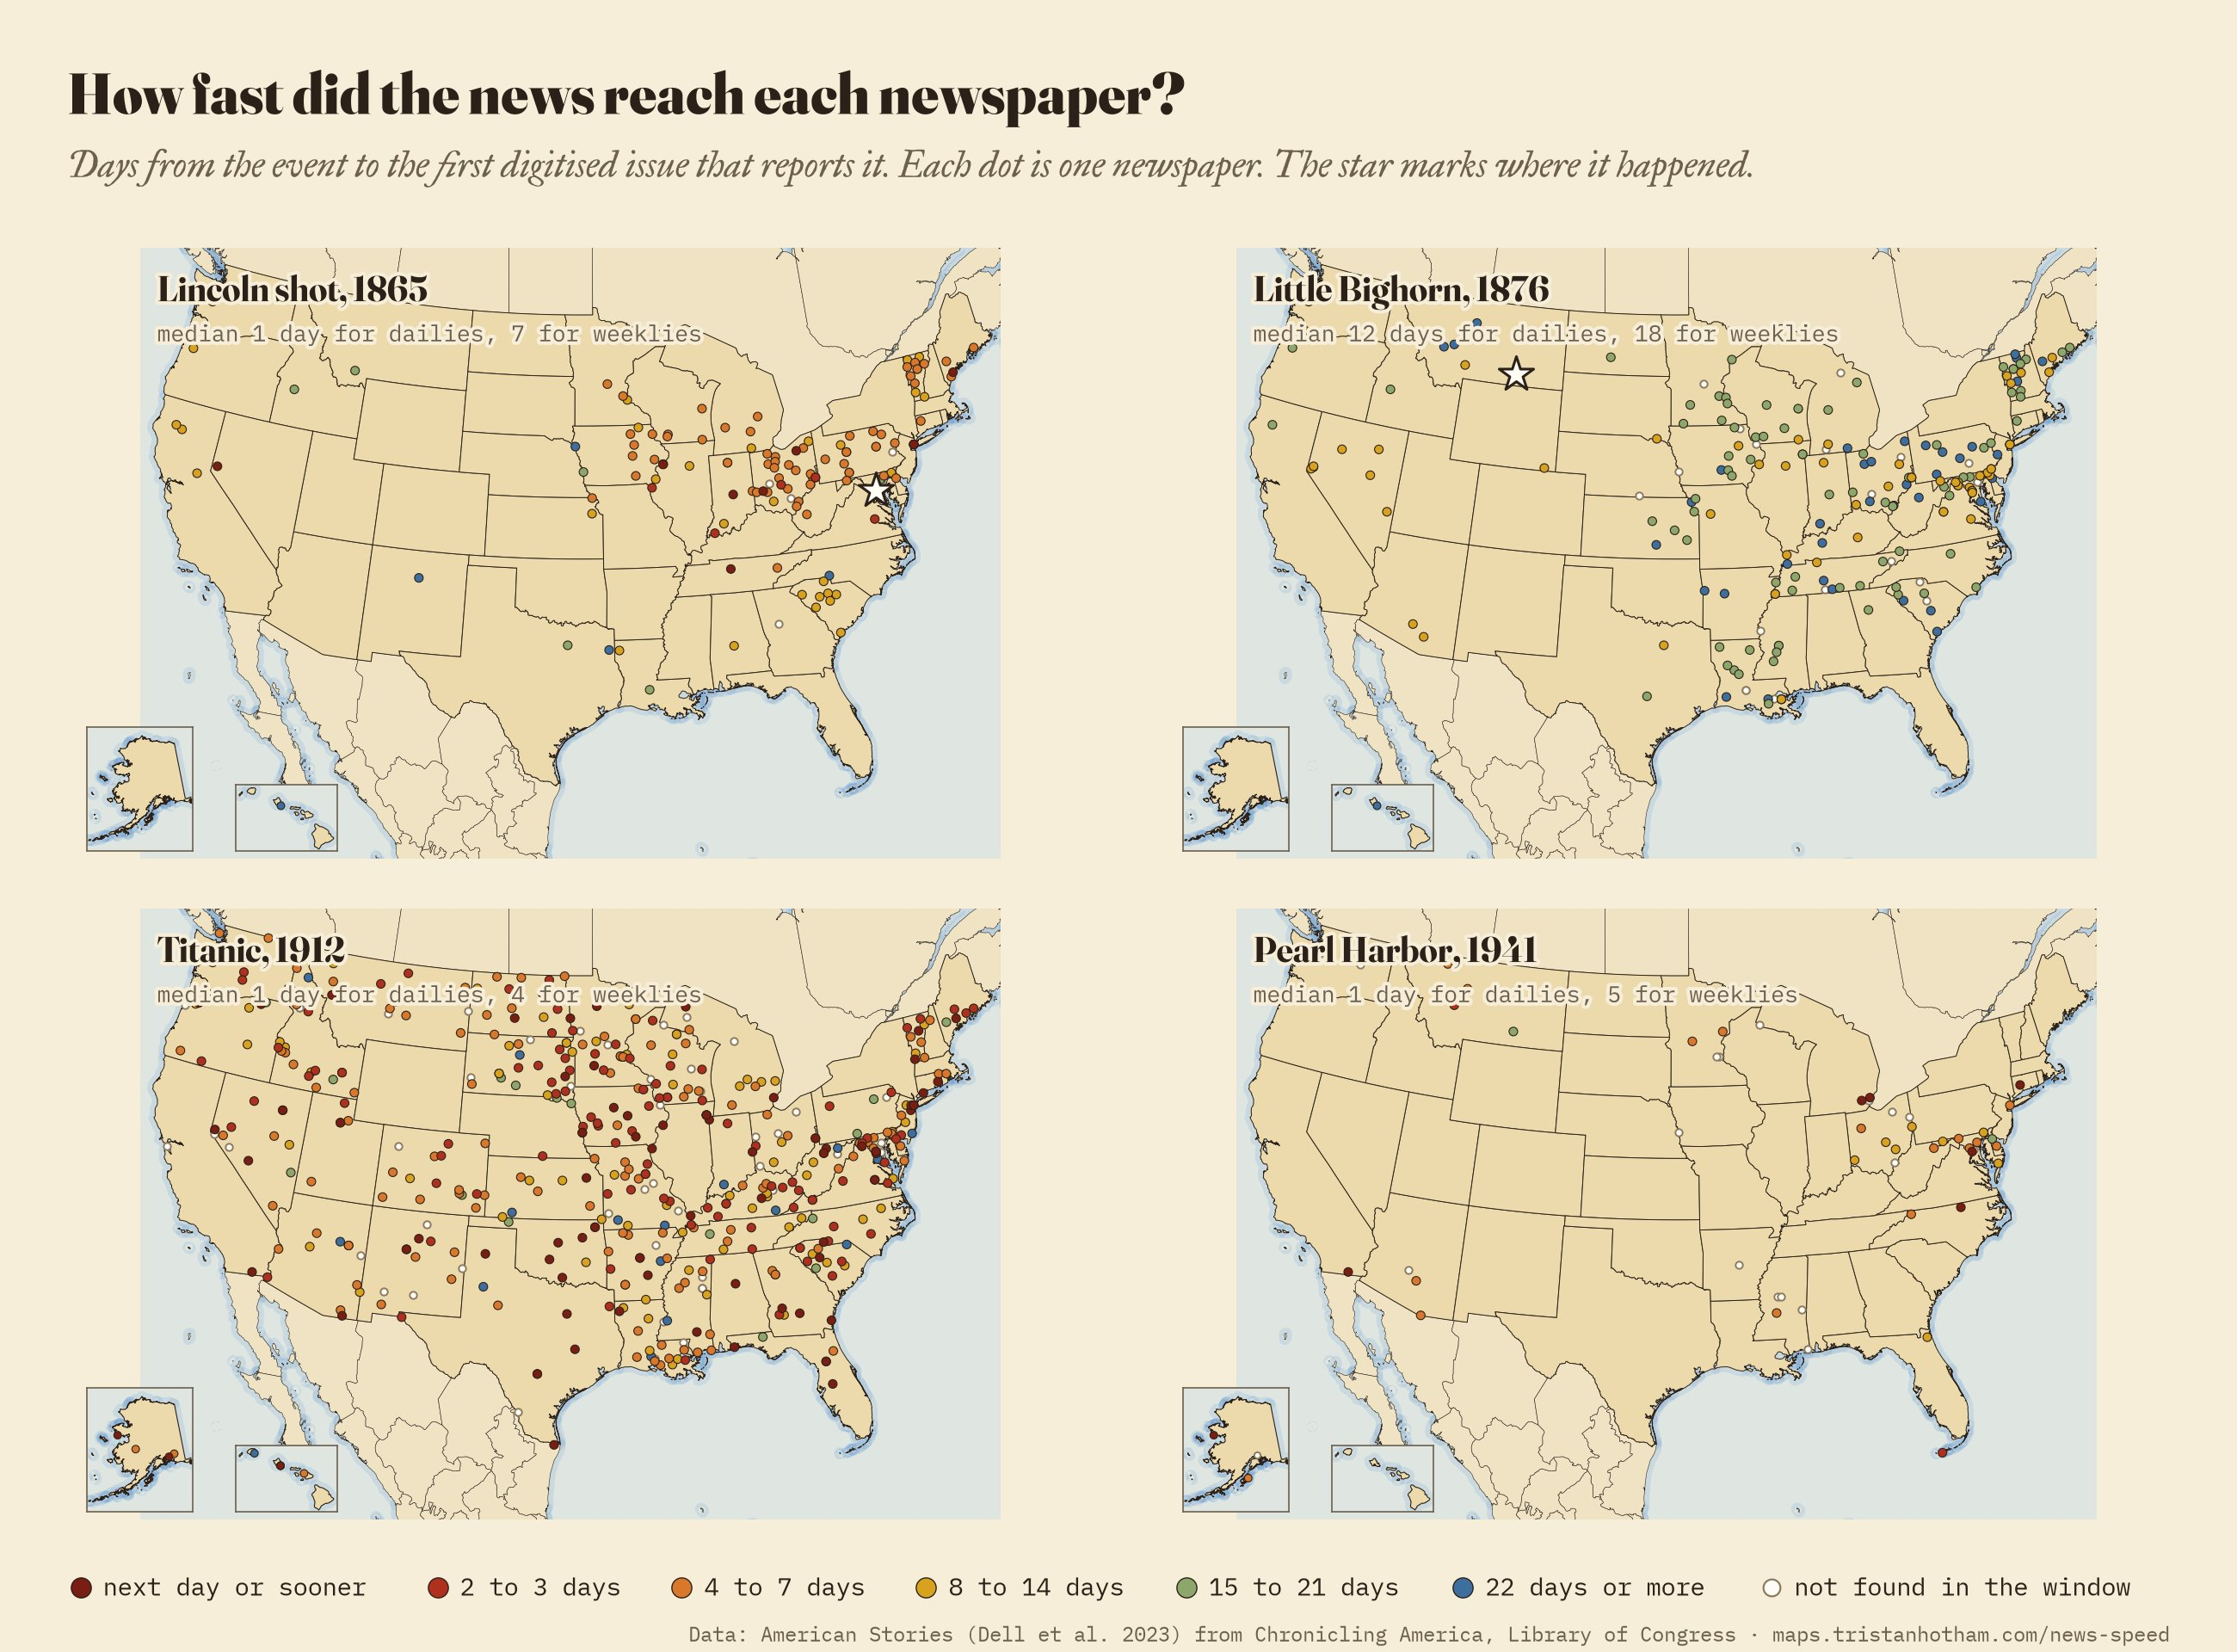
\includegraphics[width=\textwidth]{f_maps.jpg}
\caption{Days from each event to each newspaper's first digitised report. Each dot is one paper; open dots found no report in the window. Insets: Alaska and Hawaii. The star marks Ford's Theatre and the Little Bighorn battlefield.}\label{fig:maps}\end{figure}

\subsection{Dailies and weeklies}
The clearest result is how little the daily press changed. A daily that reported Lincoln's death did so after a median of 1 day; so did dailies reporting the Titanic (1) and Pearl Harbor (1). Weeklies, which are most of the sample, waited a median of 7, 4 and 5 days (Figure~\ref{fig:cadence}). The cumulative curves (Figure~\ref{fig:curves}) climb in steps as each press day comes round. Most papers missed no issue at all: 62\% of the papers that printed Lincoln's death did so in their first issue after it, as did 65\% for the Titanic and 65\% for Pearl Harbor. The median number of issues missed since each event was 0 for Lincoln, the Titanic and Pearl Harbor, and 2 for Custer.

\begin{figure}[tbp]\centering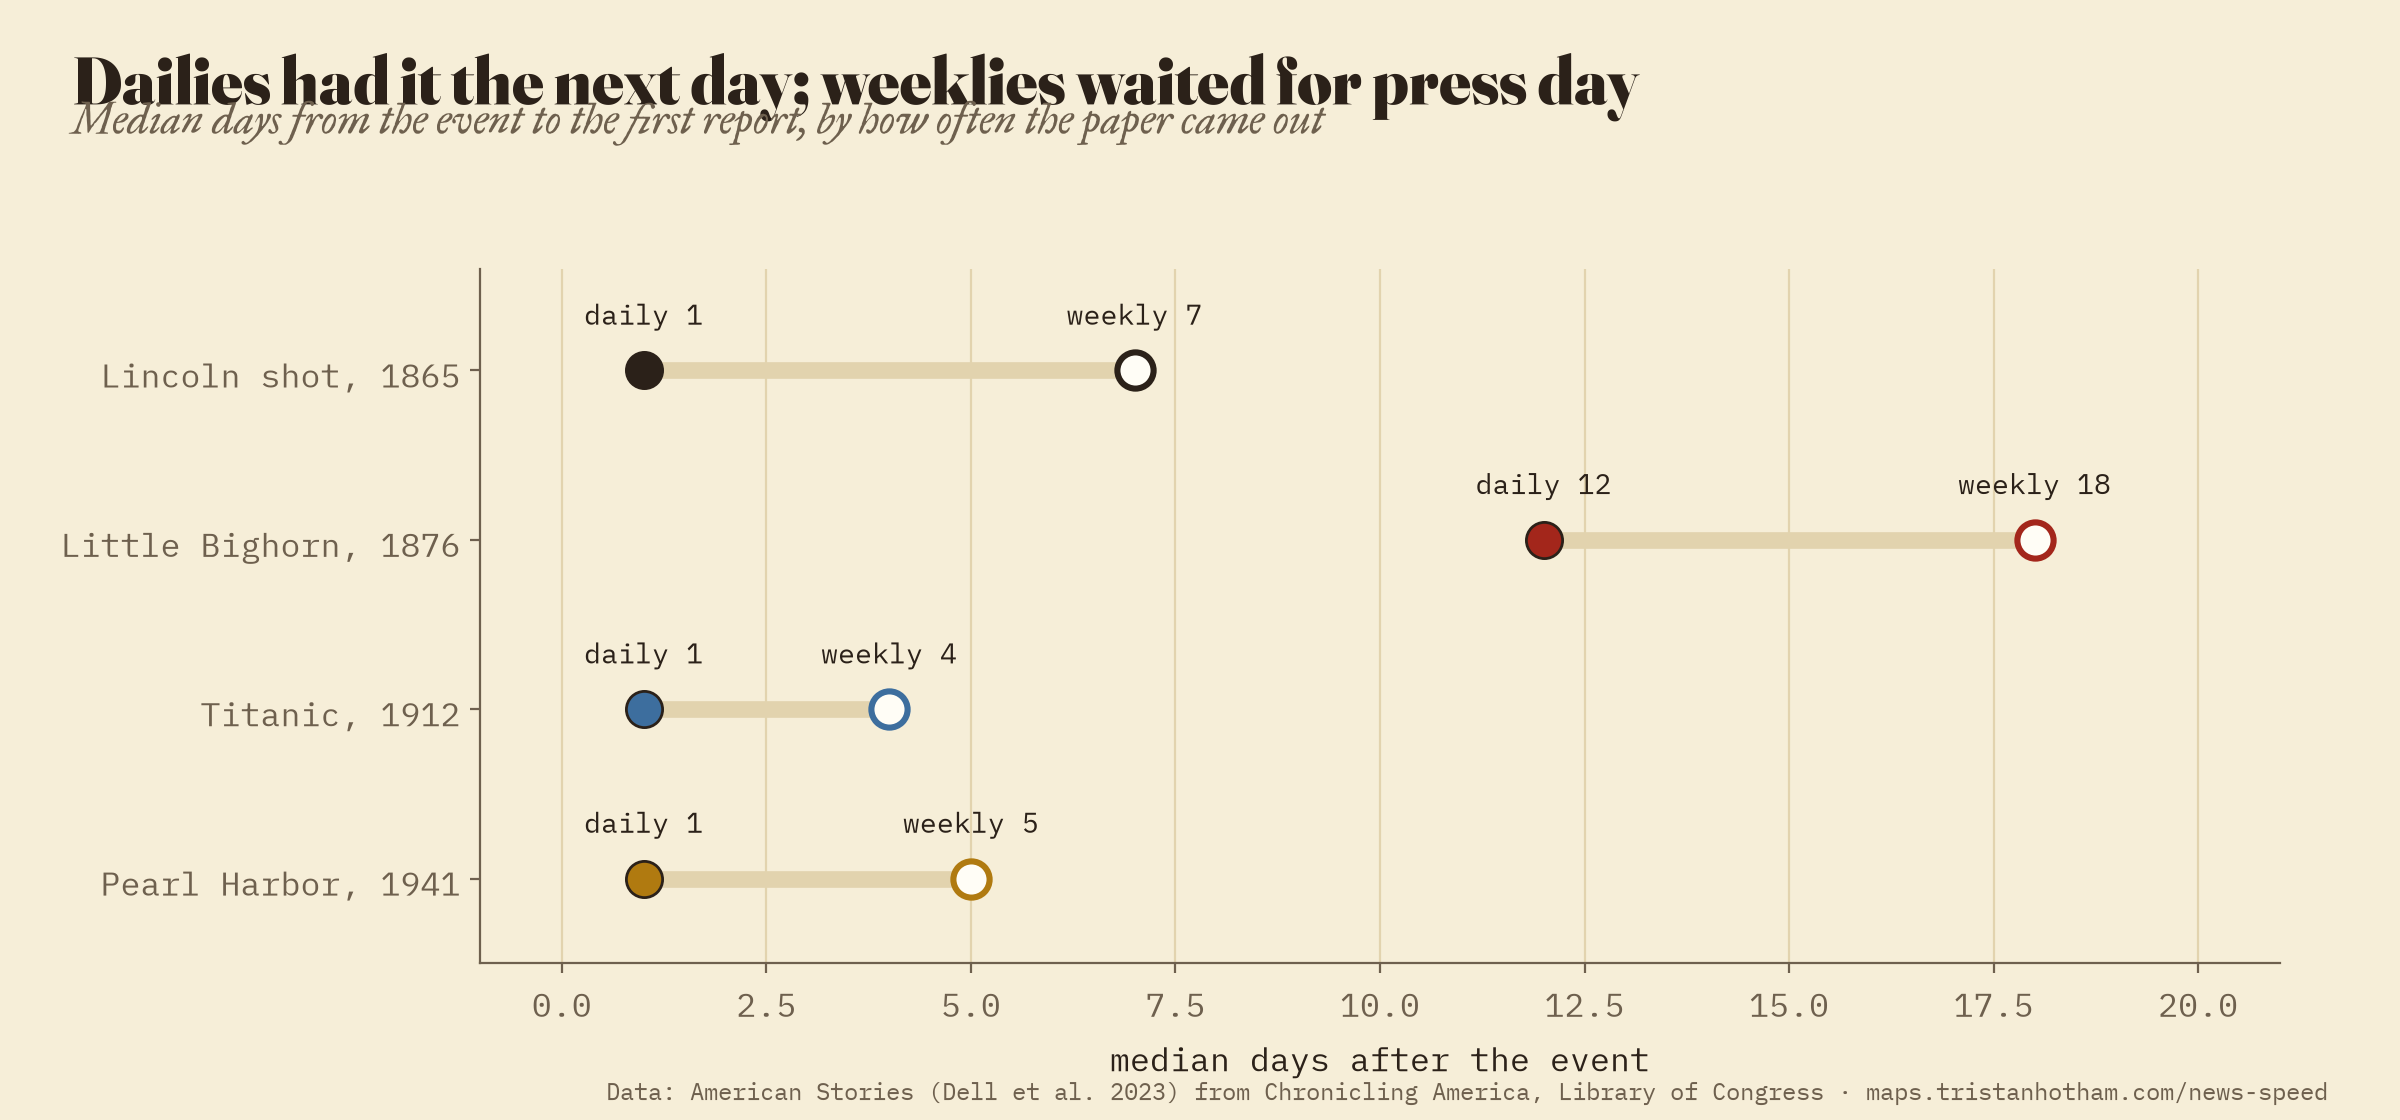
\includegraphics[width=\textwidth]{f_cadence.png}
\caption{Median days from the event to the first report, for daily papers (filled) and weekly papers (open).}\label{fig:cadence}\end{figure}
\begin{figure}[tbp]\centering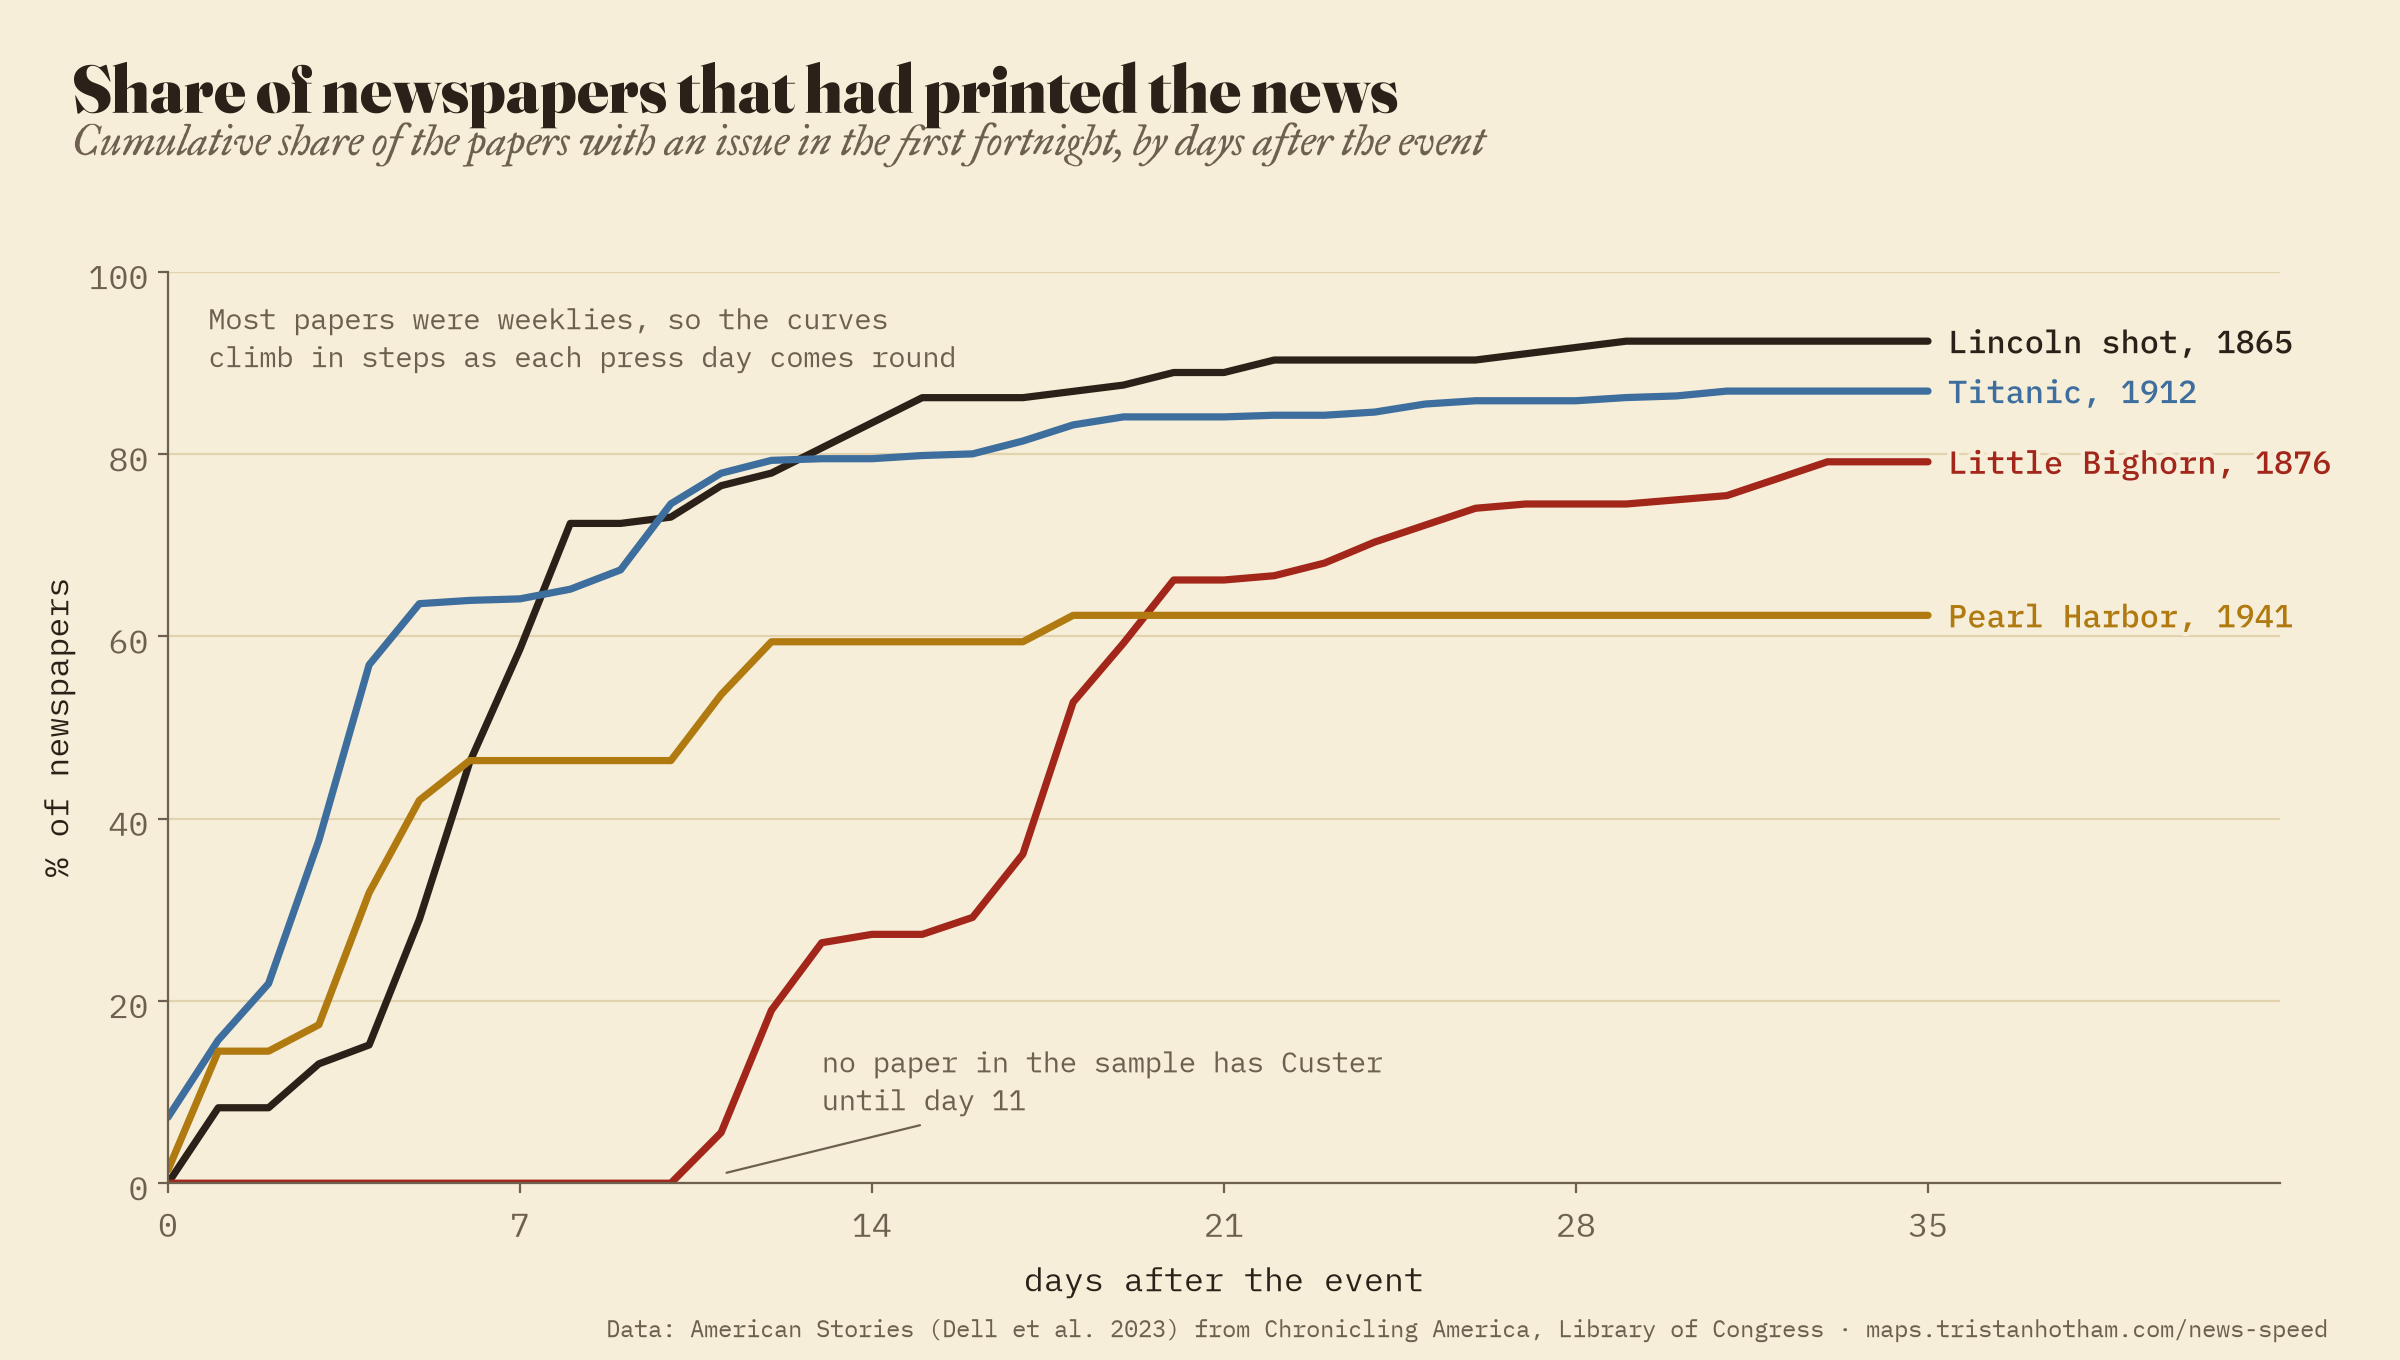
\includegraphics[width=\textwidth]{f_curves.png}
\caption{Cumulative share of papers that had printed each story, by days after the event, among papers with an issue in the first fortnight.}\label{fig:curves}\end{figure}

\subsection{Distance}
Among dailies, distance from the source barely matters (Figure~\ref{fig:distance}). The rank correlation between distance and delay among dailies was -0.16 for Lincoln (p = 0.45, 23 papers), 0.19 for the Titanic (p = 0.08, 85 papers) and -0.19 for Custer (p = 0.32). Across all papers there is a weak positive correlation for Lincoln (0.32), which comes from the slow South and far West rather than from distance as such. The striking cases are far and fast: the Gold Hill Daily News in Nevada printed Lincoln's death on 15 April 1865, 3,643 km from Washington, on the transcontinental telegraph completed in 1861; the two Honolulu dailies printed the Titanic news on 15 April 1912, 7,982 km from New York, by cable; and the Daily Alaska Empire in Juneau had Pearl Harbor on 7 December 1941.

\begin{figure}[tbp]\centering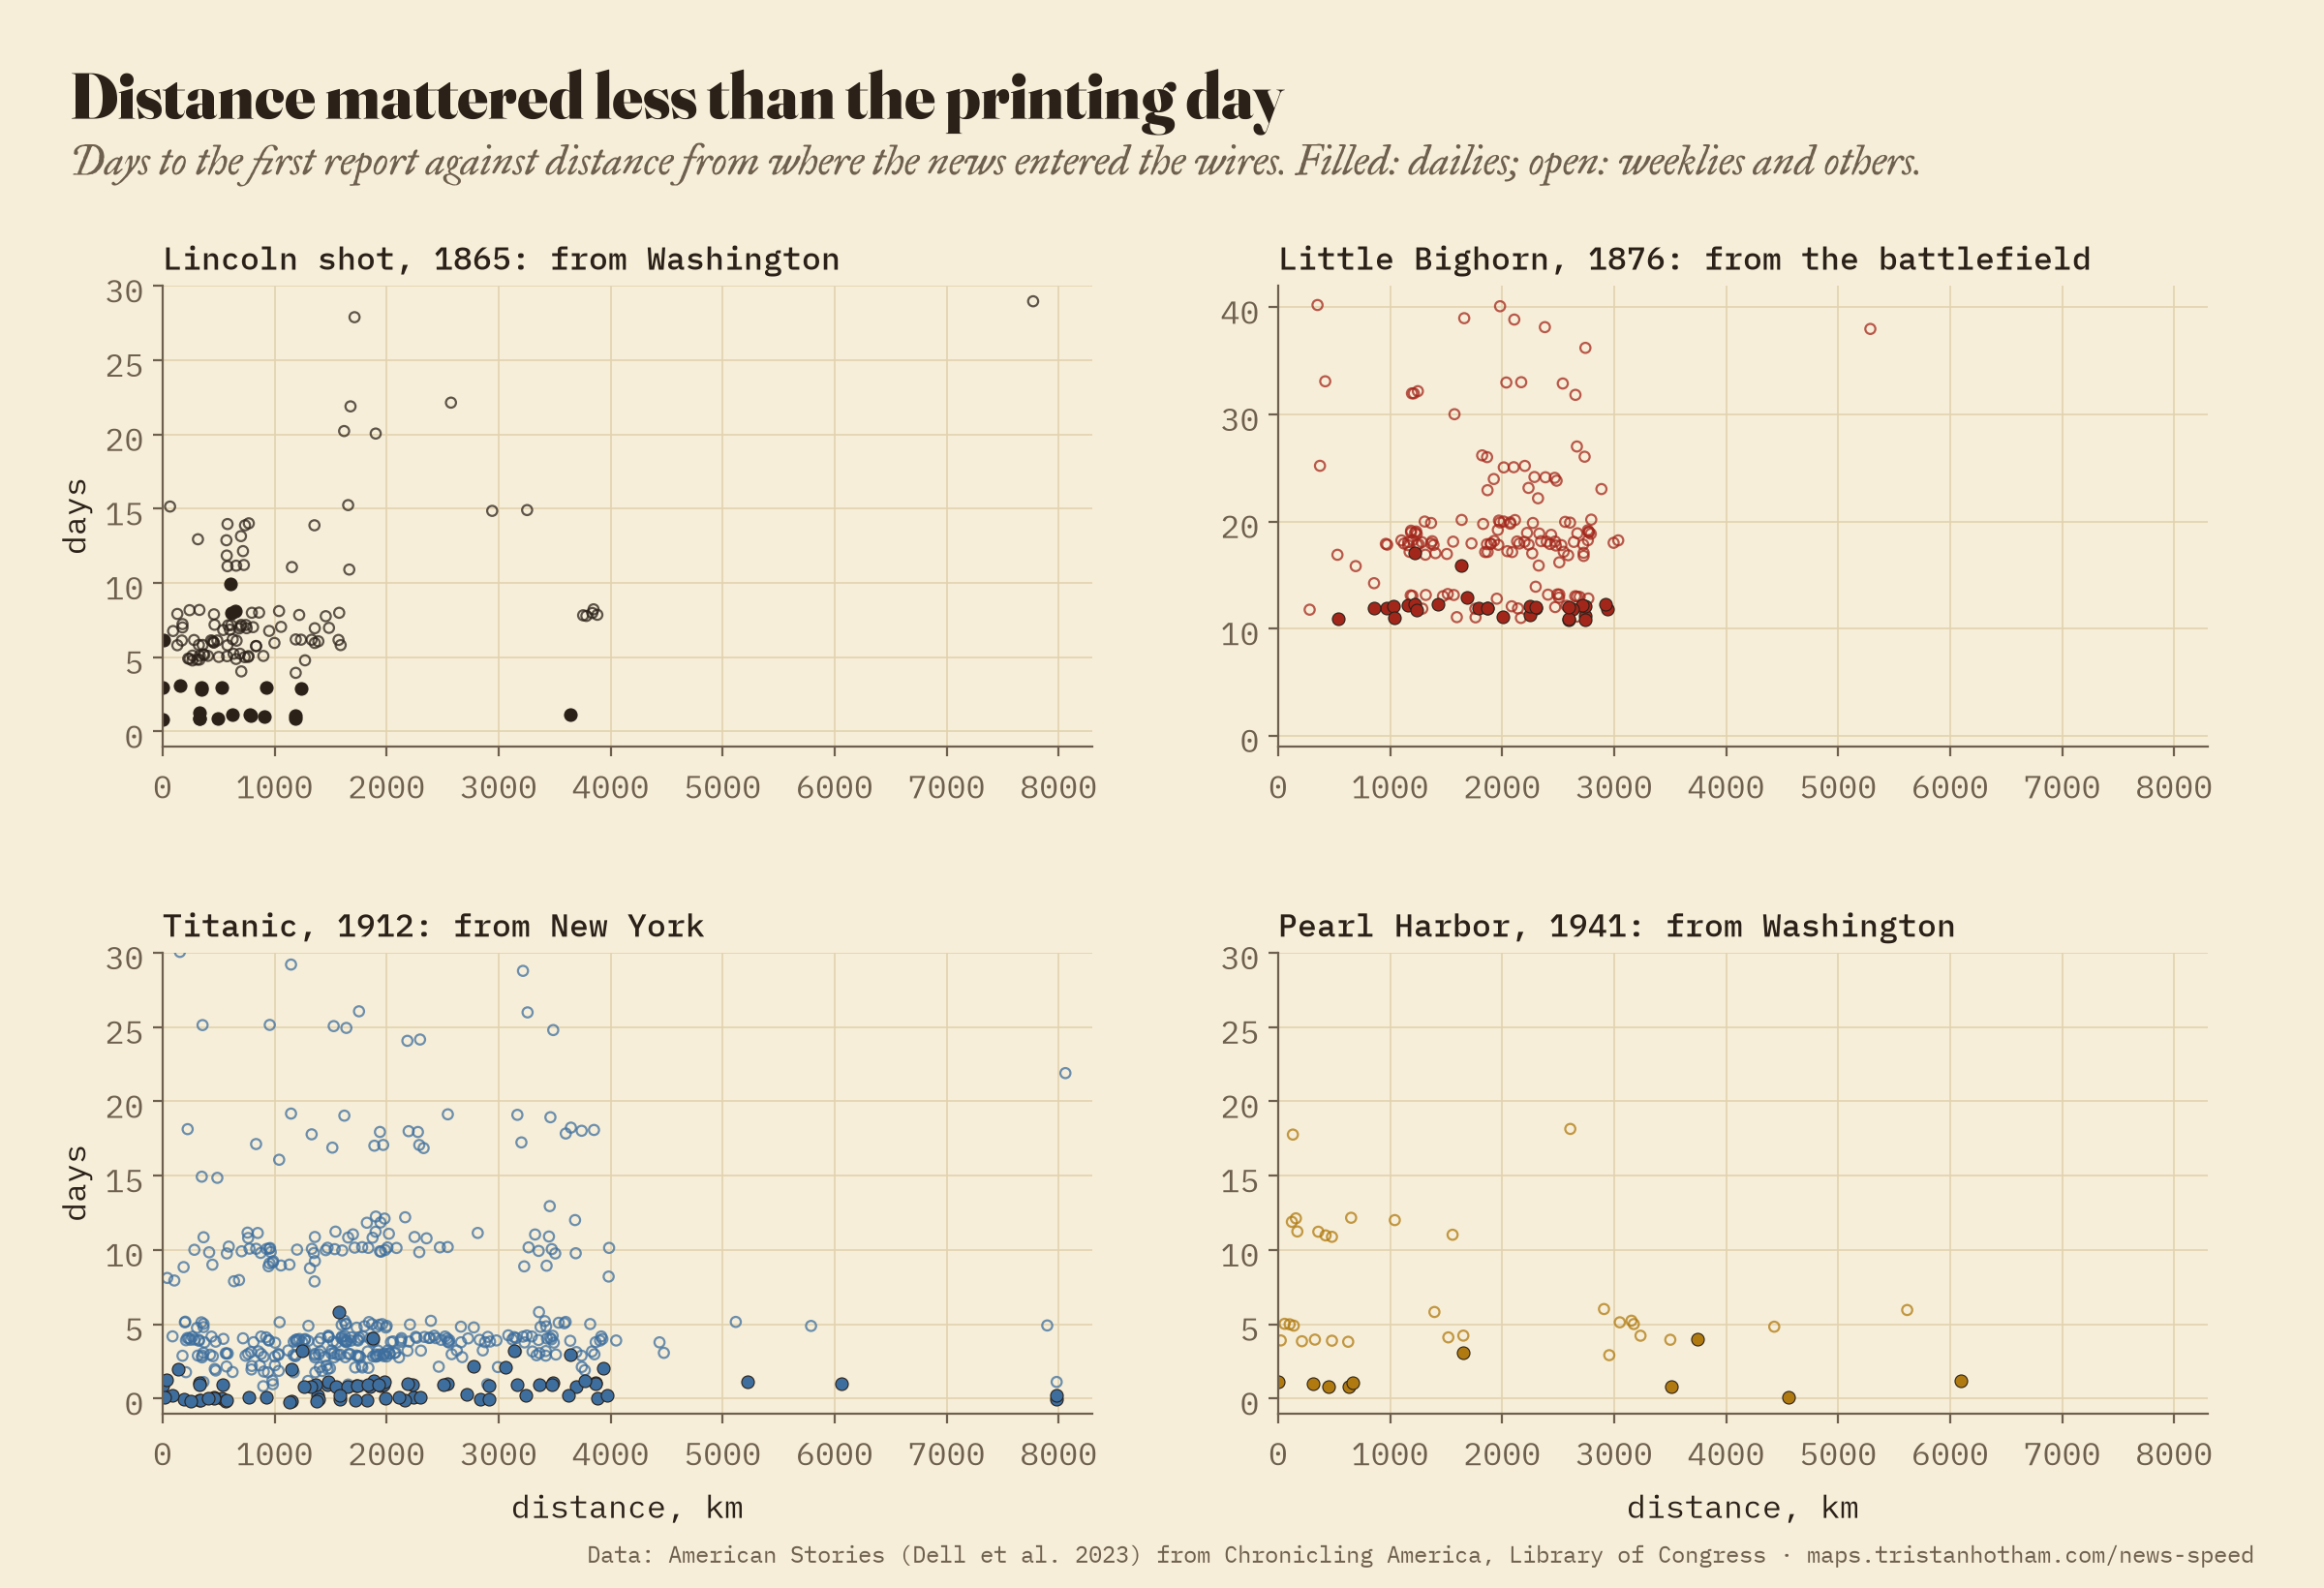
\includegraphics[width=\textwidth]{f_distance.png}
\caption{Days to the first report against distance from where the news entered the wires. Filled: dailies; open: weeklies and others. Points are jittered vertically by up to a quarter of a day.}\label{fig:distance}\end{figure}

\subsection{1865: the war}
The Civil War shaped the spread of Lincoln's death (Figure~\ref{fig:lincoln}). Papers in the eleven states of the former Confederacy took a median of 11 days (21 papers) against 6 days elsewhere (114 papers). Union-held cities in the South were fast: The Nashville Daily Union printed it on 15 April and the Richmond Whig, in a city taken by Union troops two weeks before, on 17 April. The interior was slow: South Carolina papers took a median of 10.5 days and the Texas papers three to four weeks. The Pacific Commercial Advertiser in Honolulu, then capital of the Kingdom of Hawaii and reached only by ship, printed it after 29 days.

\begin{figure}[tbp]\centering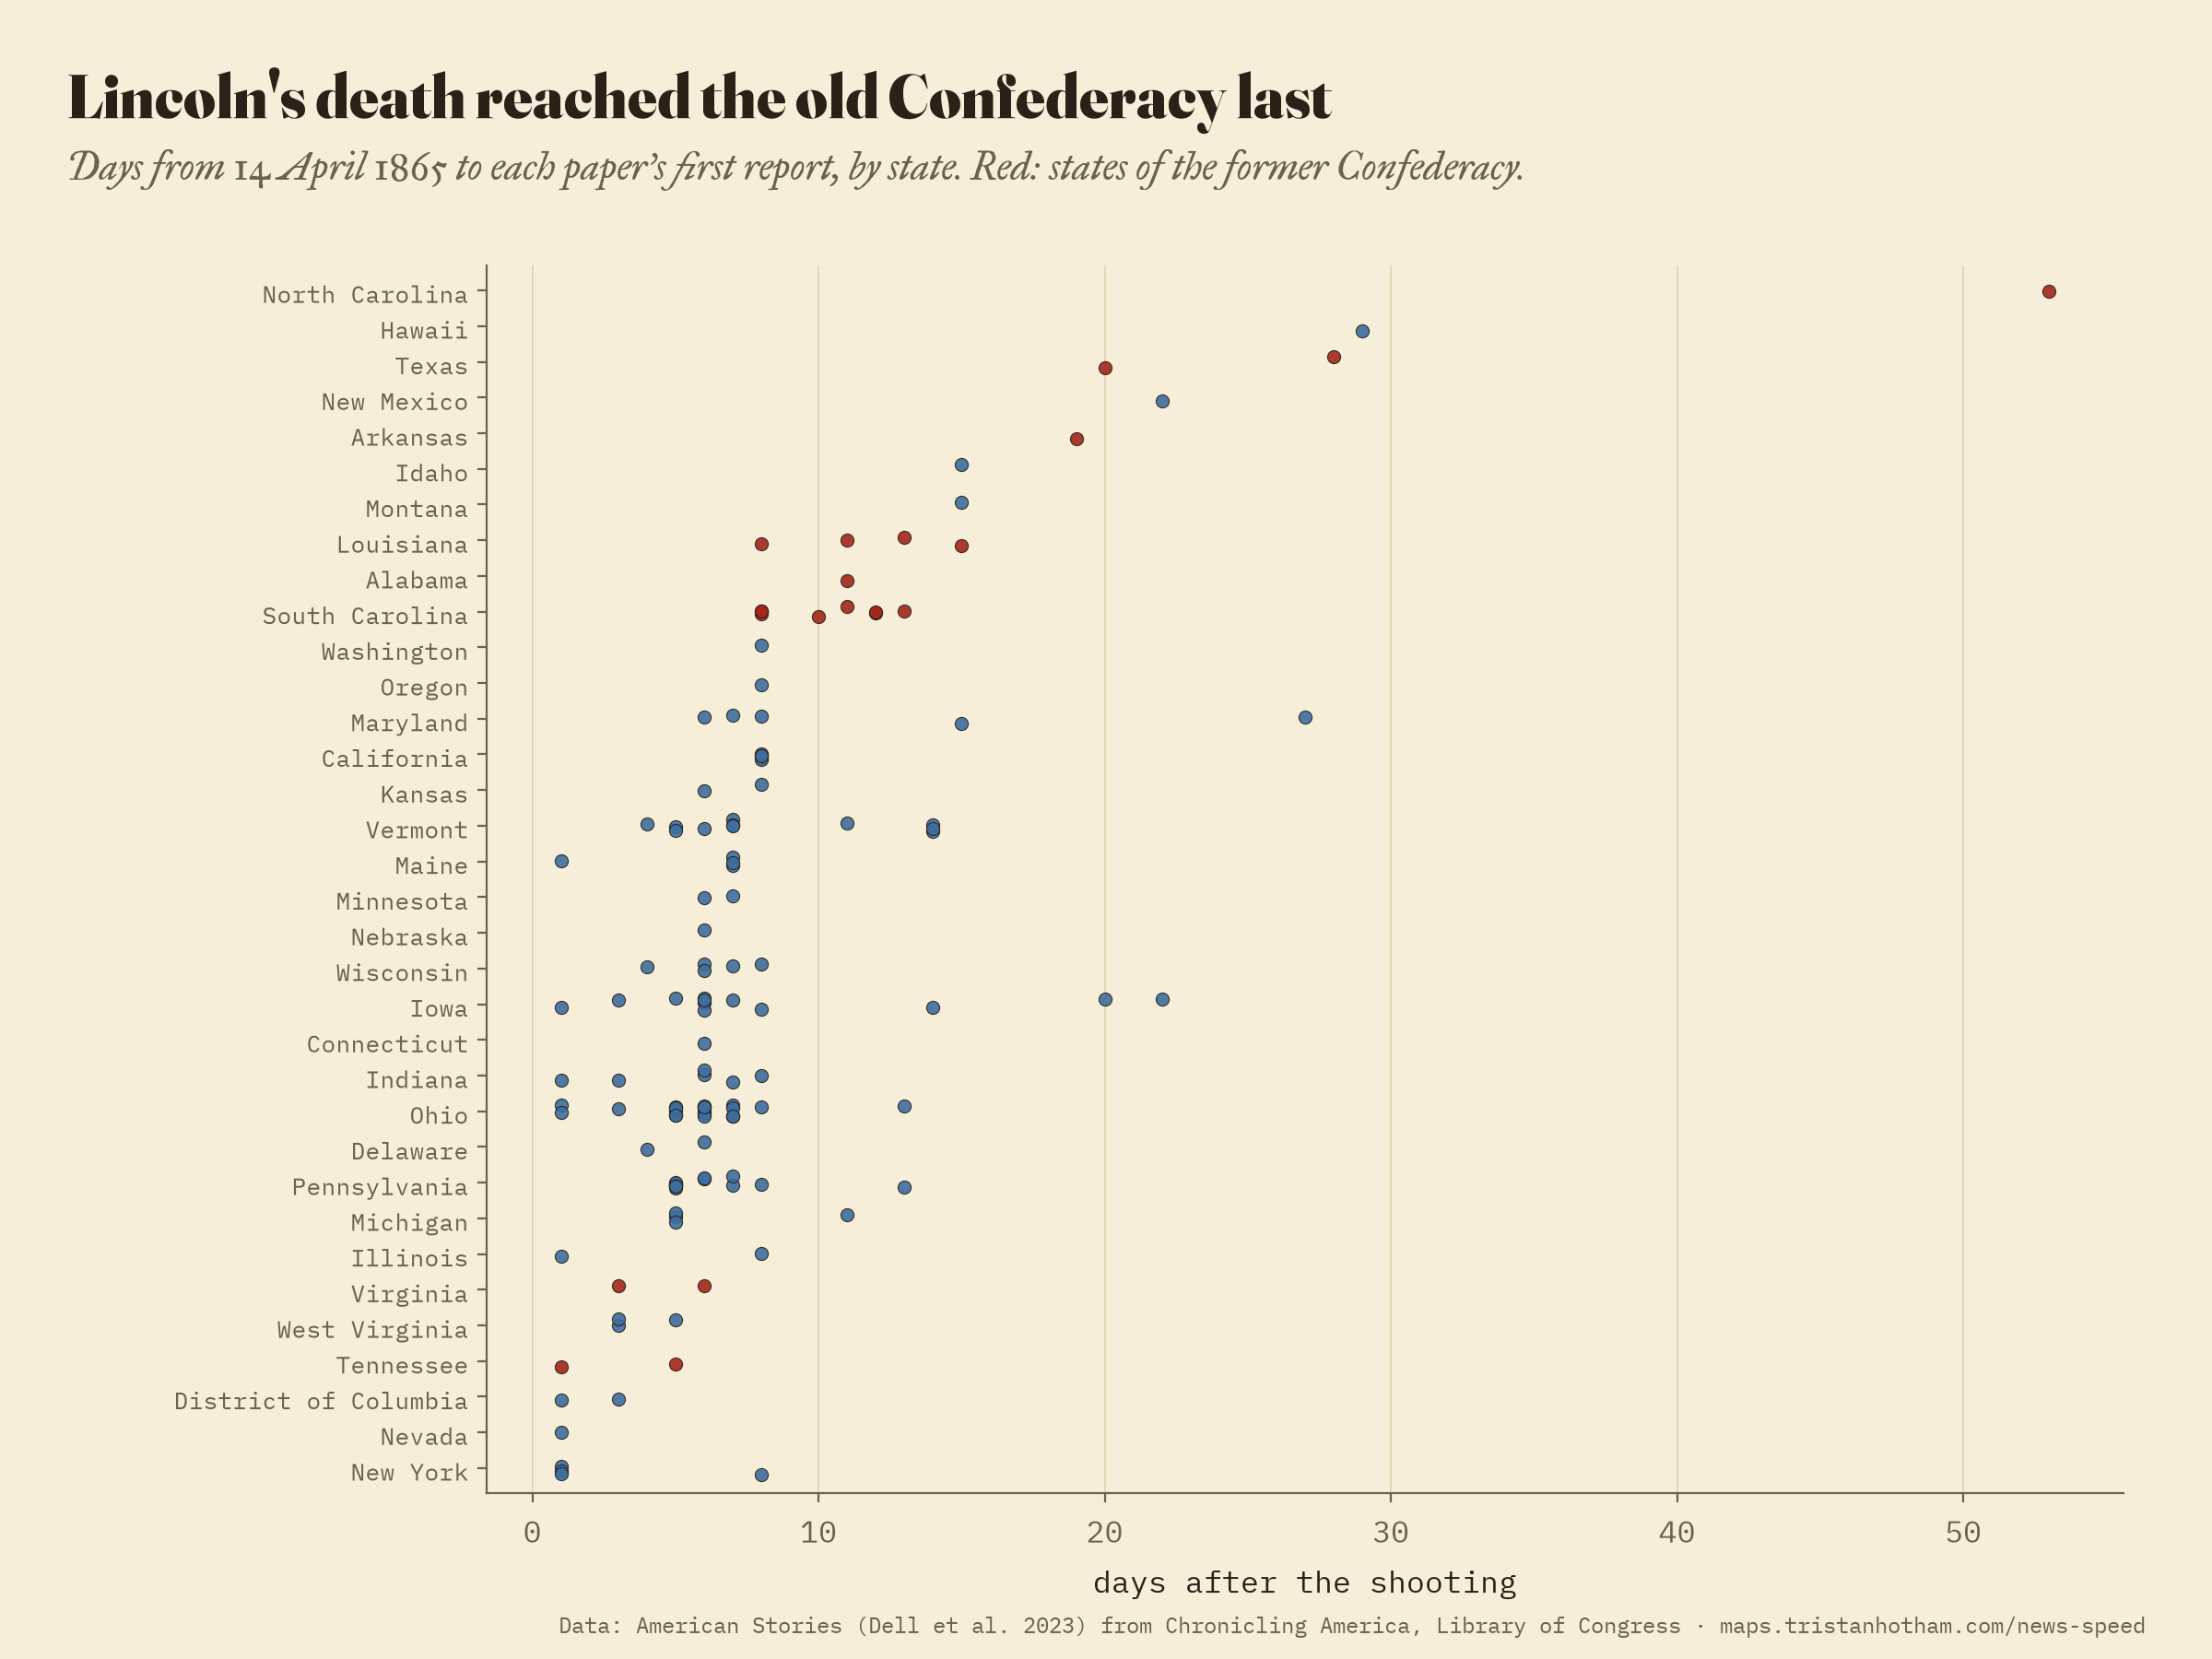
\includegraphics[width=0.92\textwidth]{f_lincoln.png}
\caption{Days from 14 April 1865 to each paper's first report of Lincoln's death, by state. Red: states of the former Confederacy.}\label{fig:lincoln}\end{figure}

\subsection{1876: the first mile}
The Little Bighorn shows where delay came from when it did come. The battle was fought on 25 June 1876; a scout carried the first word to Fort Ellis and Bozeman on 3 July, and from Montana it went east by telegraph by way of Salt Lake City, while the steamboat \textit{Far West}, carrying the wounded down the Bighorn and Yellowstone, reached Bismarck only late on 5 July. The earliest reports in the sample carry the Montana dispatches. No paper in the sample printed the news for 11 days. On 6 July it appeared in 12 papers in 9 states and territories at once, from New York and Washington to Cheyenne and Unionville, Nevada (Figure~\ref{fig:custer}). From then on, distance from the battlefield had no bearing on delay. The Montana papers in the sample show the news later than the East (median 25 days across 5 papers), but they were weeklies whose digitised text is thin; I do not read this as evidence that Montana heard last.

\begin{figure}[tbp]\centering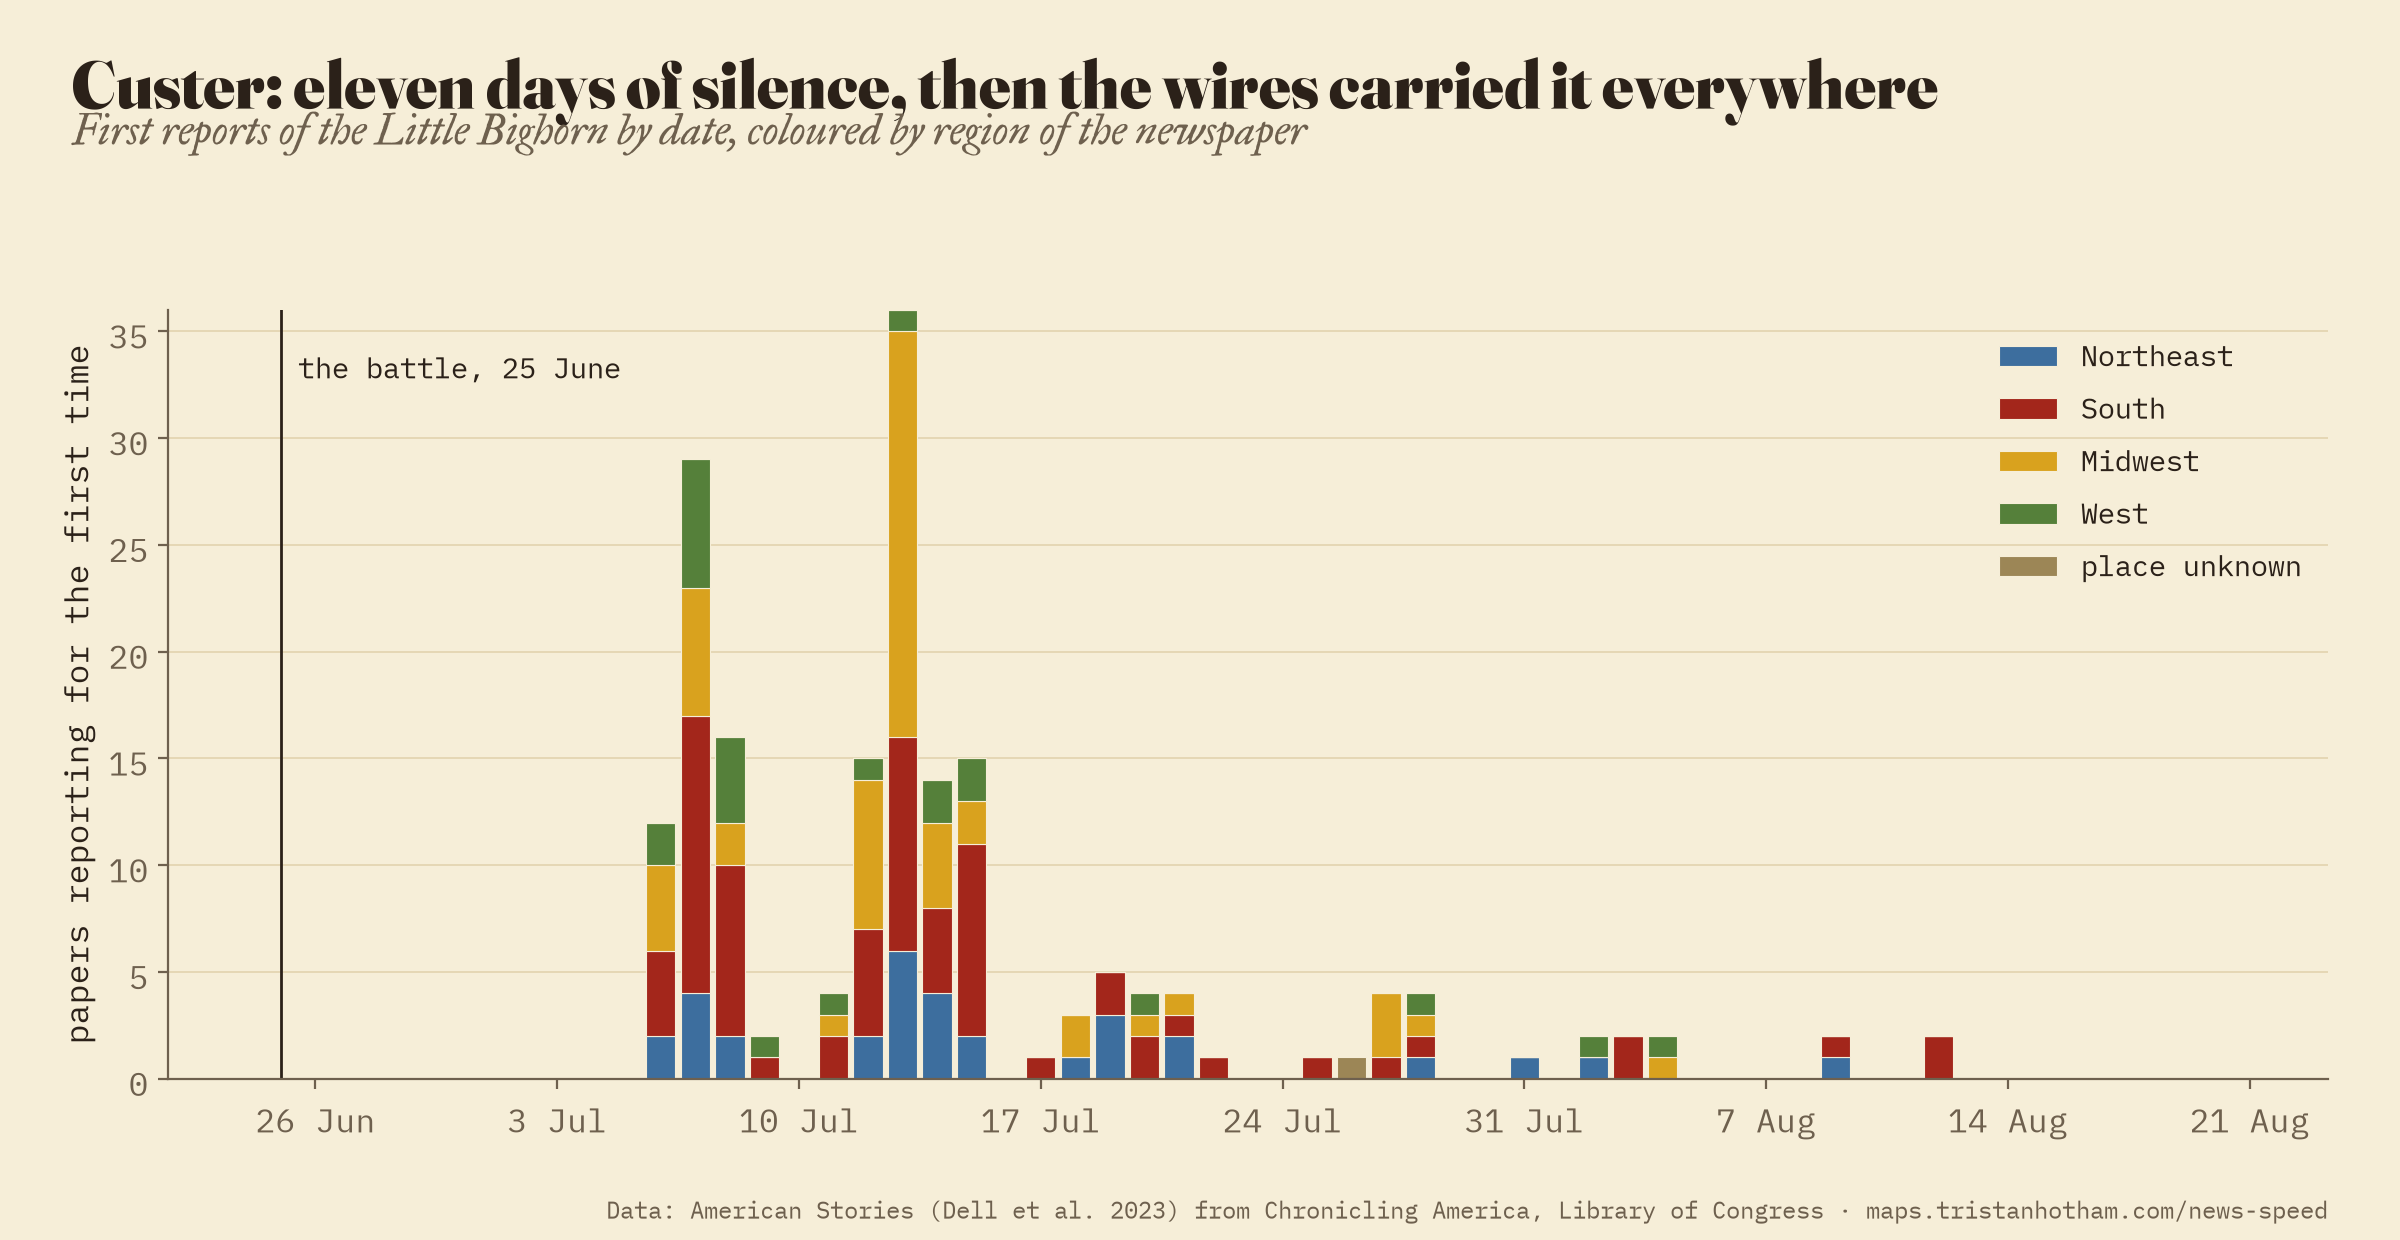
\includegraphics[width=\textwidth]{f_custer.png}
\caption{Newspapers printing Custer's defeat for the first time, by date and US census region.}\label{fig:custer}\end{figure}

\subsection{Robustness}
Counting any page that names the event on or after the floor date, without the word list, gives medians of 6, 18, 4 and 4 days, against 7, 18, 4 and 4 with it, so the conclusions do not depend on the word lists.

\section{Limitations}
The digitised papers are a sample shaped by what state libraries chose to scan for the National Digital Newspaper Program: small-town weeklies outnumber big-city dailies, some states are thickly covered and others thinly, and 1941 has few papers. The American Stories text keeps only what the layout model recognised as articles and headlines, and OCR misses words, so a paper may have printed the news an issue before the first page found here; every delay is an upper bound. Only the snippet round the first match on each page is checked, so a report below an unrelated mention on the same page can be missed. Issue dates are those printed on the paper; weeklies were often printed a day or two before their date, and some ``daily'' issues are evening editions while others are morning ones. Places are those in the paper's title and today's coordinates for that town. Finally the four events are not a random sample of news: they are the biggest stories of their years, which is exactly why every paper printed them.

\section{Conclusion}
In the digitised American press, the time it took big news to reach print was set less by distance than by two bottlenecks: getting the story from the scene to a telegraph office, and the publication rhythm of the paper that would print it. By 1865 a daily anywhere on the wire, from Maine to Nevada, printed national news the next morning; radio in 1941 did not make the daily press faster, though it surely made the public faster than the press. Where news was slow, it was slow for local reasons: a war-wrecked South in 1865, a battlefield days from the wire in 1876, the weekly press day everywhere.

\section*{Data and code availability}
The derived data (one row per newspaper and event, with dates, delays, places and the first report's snippet), the review file and all code are at \url{https://github.com/Tristan-Hotham/news-speed} and in the Zenodo record https://doi.org/10.5281/zenodo.24052721. Code MIT; text, figures and derived data CC BY 4.0. The source text is from American Stories (CC BY 4.0); places from Wikidata (CC0) and GeoNames (CC BY 4.0).

\section*{AI statement}
I wrote the text, with drafting and editing assistance from Claude (Anthropic), which also helped prepare the analysis code. I reviewed and checked all text and results.

\begin{thebibliography}{9}
\bibitem[Blondheim(1994)]{blondheim1994} Blondheim, M. (1994) \textit{News over the Wires: The Telegraph and the Flow of Public Information in America, 1844-1897}. Cambridge, MA: Harvard University Press.
\bibitem[Dell et al.(2023)]{dell2023} Dell, M., Carlson, J., Bryan, T., Silcock, E., Arora, A., Shen, Z., D'Amico-Wong, L., Le, Q., Querubin, P. and Heldring, L. (2023) American Stories: a large-scale structured text dataset of historical U.S. newspapers. \textit{arXiv} 2308.12477. \url{https://arxiv.org/abs/2308.12477}
\bibitem[GeoNames(2026)]{geonames} GeoNames (2026) GeoNames geographical database, cities500. CC BY 4.0. \url{https://www.geonames.org/}
\bibitem[Library of Congress(2026)]{chronam} Library of Congress (2026) Chronicling America: Historic American Newspapers. \url{https://chroniclingamerica.loc.gov/}
\bibitem[Pred(1973)]{pred1973} Pred, A. R. (1973) \textit{Urban Growth and the Circulation of Information: The United States System of Cities, 1790-1840}. Cambridge, MA: Harvard University Press.
\bibitem[Standage(1998)]{standage1998} Standage, T. (1998) \textit{The Victorian Internet}. New York: Walker and Company.
\bibitem[Wikidata(2026)]{wikidata} Wikidata (2026) Wikidata, the free knowledge base. CC0. \url{https://www.wikidata.org/}
\end{thebibliography}

\appendix
\section{The earliest reports}
{\footnotesize\begin{longtable}{p{2.6cm}p{4.6cm}p{3.6cm}lrr}\caption{The six earliest reports of each event, the farthest first among papers reporting on the same day. Distance in km from the news hub.}\\\toprule Event & Paper & Place & Date & Days & km\\\midrule\endfirsthead\toprule Event & Paper & Place & Date & Days & km\\\midrule\endhead
Lincoln shot, 1865 & Gold Hill daily news & Gold Hill, Nevada & 1865-04-15 & 1 & 3,643\\
Lincoln shot, 1865 & Daily Davenport Democrat & Davenport, Iowa & 1865-04-15 & 1 & 1,185\\
Lincoln shot, 1865 & The evening Argus & Rock Island, Illinois & 1865-04-15 & 1 & 1,185\\
Lincoln shot, 1865 & The Nashville daily union & Nashville, Tennessee & 1865-04-15 & 1 & 910\\
Lincoln shot, 1865 & Daily State sentinel & Indianapolis, Indiana & 1865-04-15 & 1 & 790\\
Lincoln shot, 1865 & The Portland daily press & Portland, Maine & 1865-04-15 & 1 & 775\\
\midrule
Little Bighorn, 1876 & New-York tribune & New York, New York & 1876-07-06 & 11 & 2,744\\
Little Bighorn, 1876 & The sun & New York, New York & 1876-07-06 & 11 & 2,744\\
Little Bighorn, 1876 & Wilmington daily commercial & Wilmington, Delaware & 1876-07-06 & 11 & 2,667\\
Little Bighorn, 1876 & Alexandria gazette & Alexandria, Virginia & 1876-07-06 & 11 & 2,596\\
Little Bighorn, 1876 & Evening star & Washington, District of Columbia & 1876-07-06 & 11 & 2,592\\
Little Bighorn, 1876 & The Wheeling daily intelligencer & Wheeling, West Virginia & 1876-07-06 & 11 & 2,251\\
\midrule
Titanic, 1912 & The Hawaiian star & Honolulu, Hawaii & 1912-04-15 & 0 & 7,982\\
Titanic, 1912 & Evening bulletin & Honolulu, Hawaii & 1912-04-15 & 0 & 7,982\\
Titanic, 1912 & Daily capital journal & Salem, Oregon & 1912-04-15 & 0 & 3,965\\
Titanic, 1912 & The Tacoma times & Tacoma, Washington & 1912-04-15 & 0 & 3,879\\
Titanic, 1912 & East Oregonian : E.O & Pendleton, Oregon & 1912-04-15 & 0 & 3,624\\
Titanic, 1912 & The Daily Missoulian & Missoula, Montana & 1912-04-15 & 0 & 3,246\\
\midrule
Pearl Harbor, 1941 & The Daily Alaska empire & Juneau, Alaska & 1941-12-07 & 0 & 4,559\\
Pearl Harbor, 1941 & The Nome nugget & Nome, Alaska & 1941-12-08 & 1 & 6,095\\
Pearl Harbor, 1941 & Imperial Valley press & El Centro, California & 1941-12-08 & 1 & 3,512\\
Pearl Harbor, 1941 & The Ypsilanti daily press & Ypsilanti, Michigan & 1941-12-08 & 1 & 669\\
Pearl Harbor, 1941 & Detroit evening times & Detroit, Michigan & 1941-12-08 & 1 & 635\\
Pearl Harbor, 1941 & The Waterbury Democrat & Waterbury, Connecticut & 1941-12-08 & 1 & 450\\\bottomrule\end{longtable}}
\end{document}
